%%% Globale Einstellungen und Laden von Paketen (~Bibliotheken)
\documentclass[aspectratio=169,presentation]{beamer}
%\documentclass[aspectratio=169,handout]{beamer}

\usetheme{Boadilla} % Bestimmt das gesamte Erscheinungsbild, die folgenden fand ich grundsätzlich ganz passend:
% Hannover, Singapore, Malmoe, Boadilla, CambridgeUS

\useinnertheme{default}

% setting locales
\usepackage[utf8]{inputenc}
\usepackage[T1]{fontenc}
\usepackage[ngerman]{babel}
\usepackage{lmodern}
\usepackage[locale=DE,mode=math,list-final-separator={ oder },range-phrase={ bis },scientific-notation=false,group-digits=integer]{siunitx}

% package includes
\usepackage{tikz}
\usetikzlibrary{positioning,automata}
\usepackage{xcolor}
\usepackage{listings}

%listing setup
\definecolor{pblue}{rgb}{0.13,0.13,1}
\definecolor{pgreen}{rgb}{0,0.5,0}
\definecolor{pred}{rgb}{0.9,0,0}
\definecolor{pgrey}{rgb}{0.46,0.45,0.48}
\definecolor{javared}{rgb}{0.6,0,0} % for strings
\definecolor{javagreen}{rgb}{0.25,0.5,0.35} % comments
\definecolor{javapurple}{rgb}{0.5,0,0.35} % keywords
\definecolor{javadocblue}{rgb}{0.25,0.35,0.75} % javadoc

\lstset{language=c,
	basicstyle=\ttfamily,
	keywordstyle=\color{javapurple}\bfseries,
	stringstyle=\color{javared},
	commentstyle=\color{javagreen},
	morecomment=[s][\color{javadocblue}]{/**}{*/},
	tabsize=2,
	showspaces=false,
	showstringspaces=false
}


%%% (Wahrscheinlich ziemlich dreckige) Umsetzung von Spezialframes, die nur groß den Titel beinhalten
\newcommand{\sectionframe}[1]{
	\begin{frame}
		\vfill
		\Huge
		\centering
		\usebeamercolor[fg]{title}
		#1
		\vfill
		\par
	\end{frame}
}



%%% Zentrales Festelegen von Terminnummer und Datum
\newcommand{\terminNummer}{5}
\date{\today}
%%%



\begin{document}
\title[CE Tutorium]{Tutorium zu\\Computer-Engineering\\im SS19}
\subtitle{Termin \terminNummer}
\author[Otto]{Jakob Otto}
\institute{HAW Hamburg}
\subject{CE Tutorium}
\pgfdeclareimage[height=0.5cm]{university-logo}{logo-haw-2017}
\logo{\href{http://haw-hamburg.de}{\pgfuseimage{university-logo}}}

\titlepage

%---------------------------------------------------------------------------------------------------------------------
%	Ablauf
%---------------------------------------------------------------------------------------------------------------------
\section{Was steht an?}
\begin{frame}{Ablauf}
	\begin{columns}
		\column{0.6\textwidth}
		\begin{itemize}
      \item Aufgabe 5
		\end{itemize}
		\column{0.4\textwidth}
		
\includegraphics[width=0.6\textwidth]{kratzen}
	\end{columns}
\end{frame}

%---------------------------------------------------------------------------------------------------------------------
%	Ideen für Aufgabe 1
%---------------------------------------------------------------------------------------------------------------------

\section{4-Phasen-Handshake}
\sectionframe{\href{https://users.informatik.haw-hamburg.de/~schafers/LOCAL/S19S_CE/Aufgabenzettel_Nr5_v08.pdf}{Aufgabenzettel}}

\begin{frame} {Metastabile Zustände}
  \begin{itemize}
    \item Signale sind nicht unmittelbar stabil
    \item Set-up hold-time usw.
    \item Signal kann also zur \glqq{}falschen\grqq{} Zeit abgetastet werden
    \item $\rightarrow$ Metastabile Zustände
  \end{itemize}
\end{frame}


\begin{frame} {Metastabile Zustände}
  \begin{figure}[ht]
    \centering
    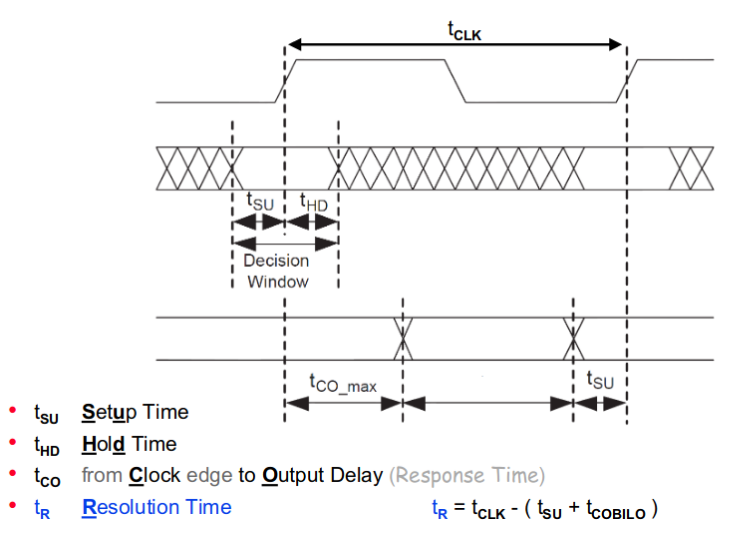
\includegraphics[width=0.7\textwidth]{figs/signalverlauf.png}
    \caption{Darstellung des clk-signals}
  \end{figure}
\end{frame}


\begin{frame} {Asynchrone kommunikation}
  \begin{itemize}
    \item Kommunikation zwischen Endpunkten oft asynchron
    \item Beide Seiten nutzen eigene Taktfrequenz
    \item Synchronisation wird benötigt
  \end{itemize}
\end{frame}


\begin{frame} {4-Phasen-Handshake}
  \begin{itemize}
    \item Kommunikationsprotokoll zum übermitteln von Daten
    \item Bidirektional über einen Datenbus
    \item Verhindert 
    \begin{itemize}
      \item Metastabile Zustände
      \item Kurzschlüsse
    \end{itemize}
  \end{itemize}
\end{frame}


\begin{frame} {Welche Leitungen?}
  Benötigt verschiedene Leitungen zur Datenübertragung
  \begin{itemize}
    \item RD/nWR - signal zum lesen/schreiben signalisieren
    \item REQ - Request vom Master zu Slave
    \item ACK/nRDY - acknowledge vom Slave zum Master
    \item Data - 16 bit Datenbus
  \end{itemize}
\end{frame}


\begin{frame} {Ablauf vom Handshake}
  Die 4 Phasen sind:
  \begin{enumerate}
    \setlength\itemsep{.5cm}
    \item Master initiiert RD/nWR = '1'\\
          Datenbus auf high-impedance\\
          REQ auf '1'
    \item Slave reagiert\\
          legt geforderte Daten auf Datenbus \\
          acknowledged (ACK = '1')
    \item Master quittiert Empfang\\
          REQ = '0'
    \item Slave nimmt Daten vom Bus\\
          Datenbus auf High-impedance
  \end{enumerate}
\end{frame}


\begin{frame} {lesender Zugriff}
  \begin{figure}[ht]
    \centering
    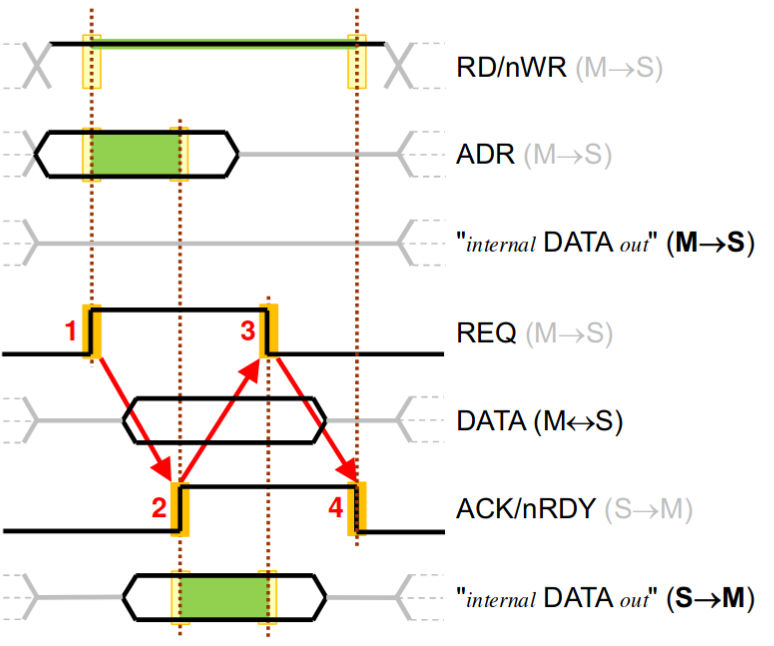
\includegraphics[height=0.7\textheight]{figs/lesen_phase.png}
    \caption{4-Phasen-Handshake lesender Zugriff}
  \end{figure}
\end{frame}


\begin{frame} [fragile]
  \begin{lstlisting}
uint16_t  rxdat;
/* wait for the fpga to be ready */
while(READY == 0);

/* setup the connection to the FPGA */
OUTPUT_DISABLE;
SET_READ;

// handle transaction by 4 phase handshake
REQ_ENABLE;
while(ACKNOWLEDGE == 0);
rxdat = (GPIOE->IDR & 0x0000FFFF);
REQ_DISABLE;
while(ACKNOWLEDGE != 0);

return rxdat;
  \end{lstlisting}
\end{frame}


\begin{frame} {Ablauf vom Handshake}
  Die 4 Phasen sind:
  \begin{enumerate}
    \setlength\itemsep{.5cm}
    \item Master initiiert RD/nWR = '0'\\
          legt Daten auf Bus \\
          REQ auf '1'
    \item Slave quittiert\\
          ACK = '1'
    \item Master setzt Bus auf High-impedance\\
          REQ = '0'
    \item slave quittiert quittung\\
          ACK = '0'
  \end{enumerate}
\end{frame}


\begin{frame} {schreibender Zugriff}
  \begin{figure}[ht]
    \centering
    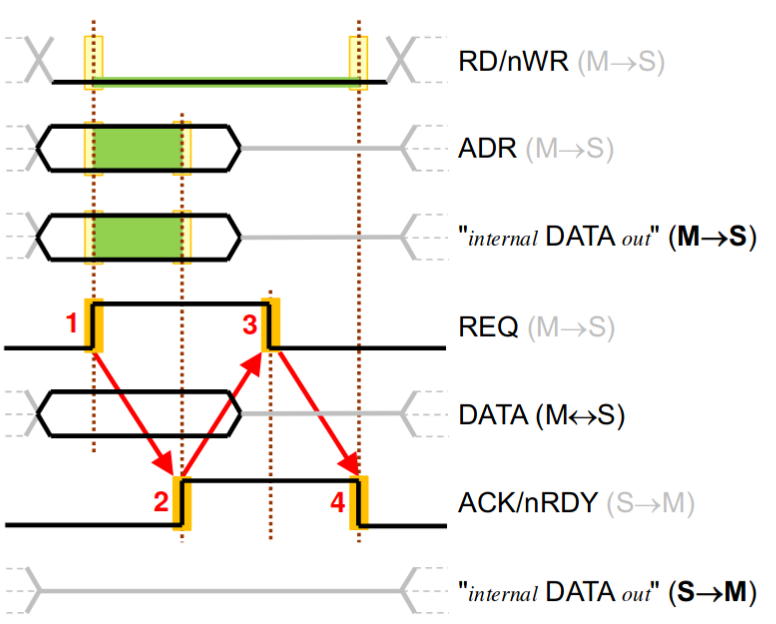
\includegraphics[height=0.7\textheight]{figs/schreibender_zugriff.png}
    \caption{4-Phasen-Handshake lesender Zugriff}
  \end{figure}
\end{frame}


\begin{frame} [fragile]
  \begin{lstlisting}
/* setup connection to the FPGA */
SET_WRITE;

OUTPUT_ENABLE;
/* set data */
GPIOE->ODR = txdat;

// handle transaction by 4 phase handshake
REQ_ENABLE;
while(ACKNOWLEDGE == 0);
REQ_DISABLE;
while(ACKNOWLEDGE != 0);
  \end{lstlisting}
\end{frame}


\begin{frame} [fragile] {FPGA-Seite}
  \begin{columns}
		\column{0.5\textwidth}
      Tri-State Treiber für Datenbus
      \begin{lstlisting} [language=vhdl]
tristate:
process (oe_s, dato_s) is
begin
  if oe_s = '1' then
    data <= dato_s;
  else
    data <= (others=>'Z');
  end if;
end process tristate;
--
dati_s <= data;
      \end{lstlisting}
    \column{0.5\textwidth}
      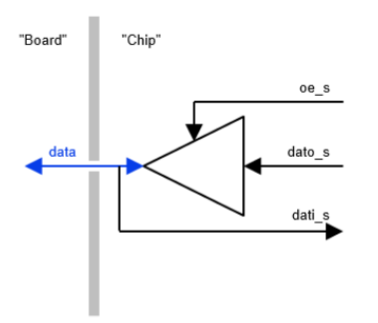
\includegraphics[width=\textwidth]{figs/tristate-treiber.png}
  \end{columns}
\end{frame}


\end{document}